\documentclass{article}


\usepackage{arxiv}

\usepackage[utf8]{inputenc} % allow utf-8 input
\usepackage[T1]{fontenc}    % use 8-bit T1 fonts
\usepackage[hidelinks]{hyperref}       % hyperlinks
\usepackage{url}            % simple URL typesetting
\usepackage{booktabs}       % professional-quality tables
\usepackage{amsfonts}       % blackboard math symbols
\usepackage{nicefrac}       % compact symbols for 1/2, etc.
\usepackage{microtype}      % microtypography
\usepackage{lipsum}
\usepackage{graphicx}
\usepackage[none]{hyphenat}
\graphicspath{ {./figures/} }


\title{Deep Learning for Medical Imaging Final Report}


\author{
    CHIH-HAO LIAO \\
    School of Forestry and Resource Conservation\\
    Graduate Institute of Biomedical Electronics and Bioinformatics\\
    National Taiwan University\\
    Taipei, Taiwan\\
    \texttt{R11625015@ntu.edu.tw} \\
    \And
    Richard LEE LAI \\
    Graduate Institute of Biomedical Electronics and Bioinformatics\\
    National Taiwan University\\
    Taipei, Taiwan \\
    \texttt{D12945021@ntu.edu.tw} \\
    \AND
    OPENAI GPT-3.5* \\
    OPENAI \\
    San Francisco, CA, USA \\
    \texttt{contact@openai.com} \\
    \AND
    *Contributed on grammar correction and translation \\
}

\begin{document}
\maketitle
\begin{abstract}
  In this study, we employ swin transformers to classify and determine the extent and existance of tumors on the chest, providing diagnostic feedback durign health inspections. The models are established by self trained and pretrained models, and the latter then further finetuned based on chest x-ray images provided better results. We show that for chest images, swin transformers offers excellent results, with an average accuracy of more than 85\%, fine-tuned model reaches 94\%. Concerning chest X-ray images, we attribute potential limitations primarily to interference stemming from the lung cavity, alongside the prominent arrangement of ribs. We aspire to further enhance our model by combine object detection before classification, enabling the automatic classificaion and labeling of the medical images and the doctors can easily figure out the target tumor cells for further process.
\end{abstract}

\keywords{Swim Transformer \and Pneumonia \and Chest X-Ray}


\section{Introduction}
\label{sec:headings}
On average, most patients need to wait for around two to three weeks for health inspection results. For those suspected of having cancer, such uncertainty can result in immense fear and anxiety. Real-time cancer detection during imaging procedures can provide immediate feedback, alleviating such negative emotions. However, the relatively high resolution of most diagnostic images makes this a difficult task. For example, digital X-ray images of breast cancer screenings often contain up to 100 MBs of information, which would require more an hour for image consolidation, image processing and tumor detection on a personal computer. This would interfere with standard operating procedures for health inspections, which are often pipelined to reduce potential bottlenecks. Therefore, we propose using the Swin transformer, a transformer-based deep learning model for inference.

\section{Methods}
\subsection{Dataset}
The dataset utilized in this study was obtained from Daniel \cite{KERMANY20181122}, who collected and labeled the chest x-ray dataset. In brief, a total of 5,232 chest X-ray images from pediatric patients were collected, comprising 3,883 images depicting pneumonia images (2,538 bacterial and 1,345 viral) and 1,349 normal images \ref{fig:chest}. The images were sourced from from 5,856 patients for training purposes. These images were sourced from 5,856 patients for training purposes. Additionally, for testing, 624 patients contributed 234 normal images and 390 pneumonia images (242 bacterial and 148 viral). By merging with the original dataset \cite{Kermany}, our dataset consisted of 5863 chest X-ray images with different resolutions, For the training, testing, and validation datasets, there were 1341, 234, and 8 images of normal patients and 3875, 390, and 8 images of pneumonia patients, respectively.

\begin{figure}[!htb]
  \centering
  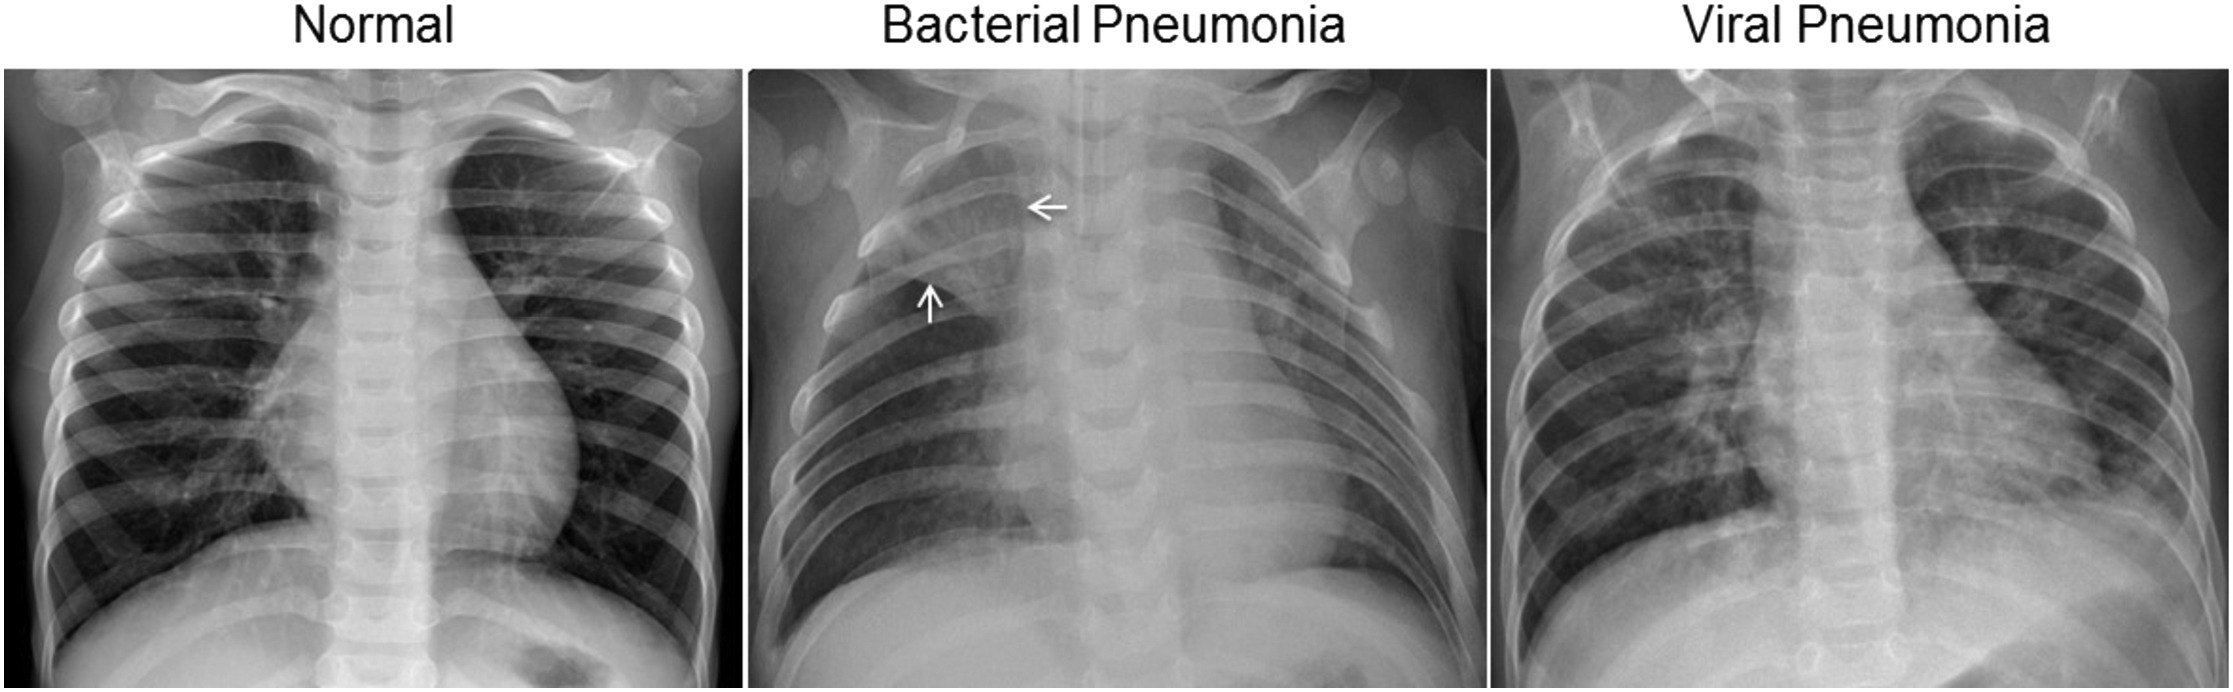
\includegraphics[width=0.8\textwidth]{chest.jpg}
  \caption{Illustrative Examples of Chest X-Rays in Patients with Pneumonia.}
  \label{fig:chest}
\end{figure}

\subsection{Model}
The Swin Transformer is a type of Vision Transformer designed for image classification and other vision tasks. It introduces a hierarchical architecture that processes images at multiple scales using shifted windows for efficient computation. This approach allows the model to handle high-resolution images and capture local context effectively. Compared with the original Vision Transformer, the Swin Transformer enables the model to capture more detailed information and achieve better performance on various vision benchmarks.

The Swin Transformer consists of four modules, each with a varying number of layers. The first module processes the input image at the original resolution, while the subsequent modules process the image at a reduced resolution. This hierarchical architecture enables the model to capture information at multiple scales and achieve state-of-the-art performance on various vision benchmarks. The Swin Transformer balances computational efficiency with high accuracy, making it suitable for a range of computer vision applications.

The hierarchical nature also enables the model to achieve state-of-the-art performance on various vision benchmarks, including image classification, object detection, and semantic segmentation. The Swin Transformer balances computational efficiency with high accuracy, making it suitable for a range of computer vision applications. In our study, the baseline model that we used is from Microsoft swin transformer v1 \cite{liu2021swin}, and the model structure that we used from pytorch is swin transformer v2 base \cite{liu2022swin}, and the pre-trained model that we used on Hugging Face is inherited from the Microsoft swinv2-tiny-patch4-window8-256.\cite{liu2022swin}.

\begin{figure}[!htb]
  \centering
  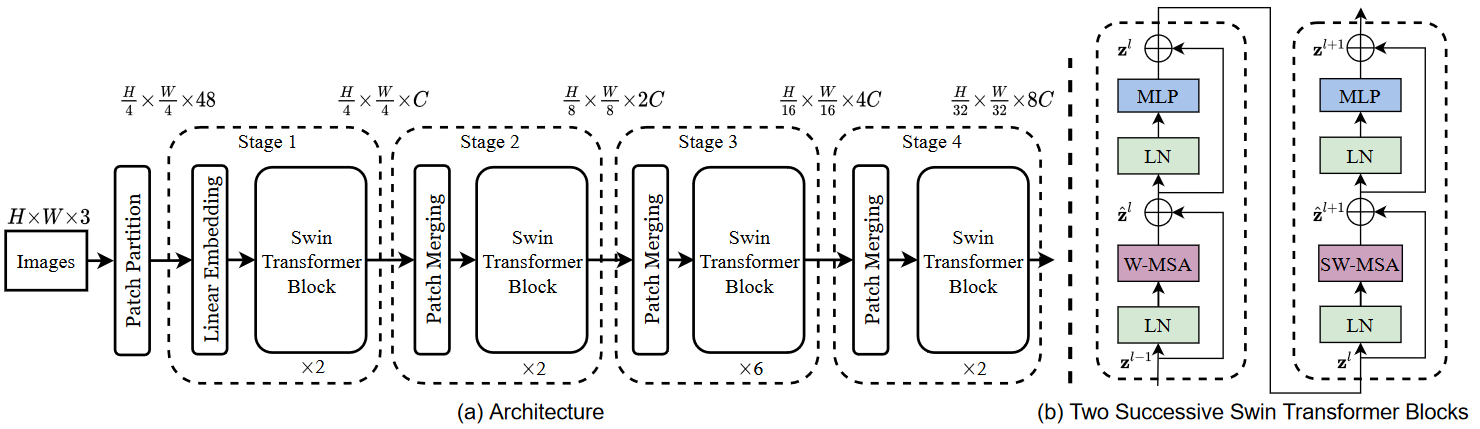
\includegraphics[width=0.8\textwidth]{swin_transformer.png}
  \caption{Architecture of Swin (shifted window) transformer. The Swin transformer consists of four modules, each with a varying number of layers.}
\end{figure}

\subsection{Preprocessing}
For the training data, a series of transformations are applied to augment the dataset and improve model generalization. Firstly, images are resized to match the dimensions expected by the feature extractor, which is 256\*256. Then, a random horizontal flip is applied, horizontally flipping images randomly to augment the dataset with mirrored versions. Following this, images are randomly rotated up to 15 degrees to further diversify the dataset. Subsequently, the transformed images are converted into PyTorch tensors. Finally, normalization is performed using the mean and standard deviation of the image dataset provided by the feature extractor. For the validation and testing dataset, only resize and normalization are applied to them. The self-trained model is normalized with pre-trained weights of ImageNet, and the fine-tuned model is applied using the mean and standard deviation of the image dataset provided by the feature extractor.

\section{Results}
The models undergo testing on the test dataset to assess their performance, with the outcomes revealing key classification metrics for each class beforehand. The findings are presented in Table \ref{tab:table1} and Table \ref{tab:table2} below.

\subsection{Self trained model}
Based on the evaluation metrics presented in Table \ref{tab:table1}, our self-trained model demonstrates promising performance in classifying chest X-ray images into two classes: NORMAL and PNEUMONIA. The precision, recall, and F1 score for each class provide insights into the model's ability to correctly identify instances of each class.

For the NORMAL class, the model achieves a precision of 99.3\%. However, the recall for this class is lower at 61.5\%, suggesting that the model misses identifying a considerable portion of actual NORMAL instances. Consequently, the F1-score, which balances precision and recall, is 76.0\% for this class.

In contrast, for the PNEUMONIA class, the model exhibits a precision 81.2\%, which means less instances predicted as PNEUMONIA are indeed NORMAL cases. The high recall of 99.7\% indicates that the model effectively captures almost all true PNEUMONIA instances. Consequently, the F1-score for this class is notably higher at 89.5\%, reflecting the model's balanced performance in identifying PNEUMONIA cases.

The overall accuracy indicating that it correctly classifies approximately 85.4\% of the instances in the dataset. The macro average F1-score, which considers the balanced performance across both classes, is 82.8\%, while the weighted average F1-score, which accounts for class imbalance, is 84.5\%.

\begin{table}[!htb]
  \caption{Classification report for the self-trained model.}
  \centering
  \begin{tabular}{lllll}
    \toprule
    \cmidrule(r){1-4}
                 & Precision & Recall & F1-Score & Support \\
    \midrule
    NORMAL       & 99.3\%    & 61.5\% & 76.0\%   & 234.0   \\
    PNEUMONIA    & 812\%     & 99.7\% & 89.5\%   & 390.0   \\
    Accuracy     &           &        & 85.4\%   & 624.0   \\
    Macro avg    & 90.3\%    & 80.6\% & 82.8\%   & 624.0   \\
    Weighted avg & 88.0\%    & 85.4\% & 84.5\%   & 624.0   \\
    \bottomrule
  \end{tabular}
  \label{tab:table1}
\end{table}

\subsection{Fine-tuned model from pre-trained model}
Based on the results obtained from our fine-tuned model, we present a comprehensive evaluation of its performance in classifying pneumonia cases from chest X-ray images. The Table \ref{tab:table2} illustrates the result.

Our model achieves an impressive precision of 97.1\% for NORMAL cases, indicating its ability to correctly identify true negative instances. Moreover, with a recall of 85.9\%, our model demonstrates a strong capacity to capture the majority of true positive pneumonia cases. The corresponding F1-score of 91.2\% further solidifies the model's balanced performance in terms of precision and recall for NORMAL class prediction.

For the PNEUMONIA class, our model maintains a high precision of 92.1\%, signifying its proficiency in correctly labeling positive instances. Additionally, a remarkable recall of 98.5\% suggests the model's capability to effectively identify the vast majority of pneumonia cases present in the dataset. This is reflected in the F1-score of 95.2\%, indicating a harmonious balance between precision and recall for PNEUMONIA class prediction.

The overall accuracy of our fine-tuned model is reported at 93.7\%, underscoring its ability to make correct classifications across both classes. The macro-average F1-score of 93.2\% and the weighted-average F1-score of 93.7\% further validate the model's robust performance across all classes, considering their respective support values.

These results demonstrate the effectiveness of our fine-tuned model in accurately classifying pneumonia cases from chest X-ray images. The high precision and recall values attained for both classes underscore the model's potential for clinical application in assisting radiologists with accurate diagnosis and patient management. Moreover, the accuracy is better than the previous studies \cite{KERMANY20181122}, which is 92.8\%.

\begin{table}[!htb]
  \caption{Classification report for fine-tuned model based on pre-trained model.}
  \centering
  \begin{tabular}{lllll}
    \toprule
    \cmidrule(r){1-4}
                 & Precision & Recall & F1-Score & Support \\
    \midrule
    NORMAL       & 97.1\%    & 85.9\% & 91.2\%   & 234.0   \\
    PNEUMONIA    & 92.1\%    & 98.5\% & 95.2\%   & 390.0   \\
    Accuracy     &           &        & 93.7\%   & 624.0   \\
    Macro avg    & 94.6\%    & 92.2\% & 93.2\%   & 624.0   \\
    Weighted avg & 94.0\%    & 93.8\% & 93.7\%   & 624.0   \\
    \bottomrule
  \end{tabular}
  \label{tab:table2}
\end{table}

\subsection{Confusion matrix}

From these results below, including Figure \ref{fig:conf1} and \ref{fig:conf2}, it's evident that the model performs well in terms of true positives and true negatives, indicating a good ability to distinguish between normal and pneumonia cases. However, the presence of false positives and false negatives suggests that there is room for improvement, particularly in reducing false positives to avoid unnecessary concern or treatment.

\begin{figure}[!htb]
  \begin{minipage}[t]{0.45\textwidth}
    \centering
    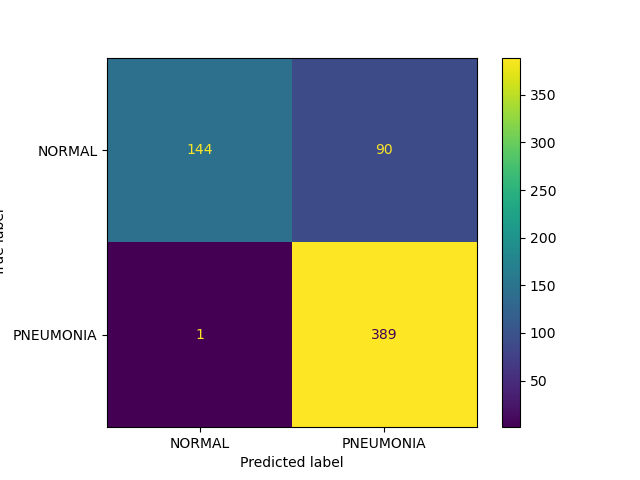
\includegraphics[width=\linewidth]{./results_train/confusion_matrix.png}
  \caption{The confusion matrix of self trained model.}
  \label{fig:conf1}
  \end{minipage}
  \hfill
  \begin{minipage}[t]{0.45\textwidth}
    \centering
    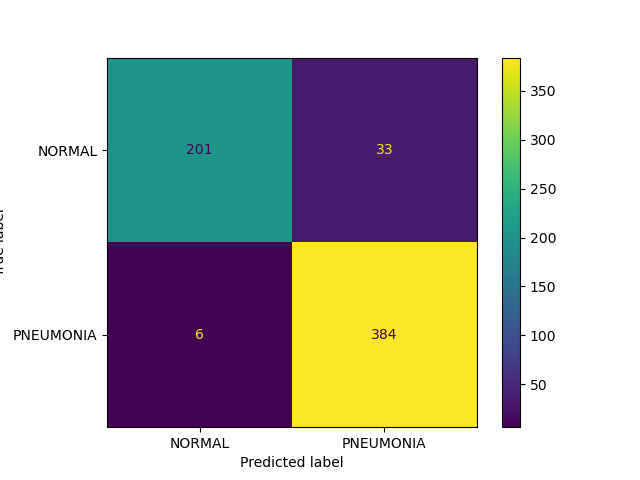
\includegraphics[width=\textwidth]{./results/image/confusion_matrix.png}
  \caption{The confusion matrix of the fine-tuned model based on pre-trained model.}
  \label{fig:conf2}
  \end{minipage}
\end{figure}

To assess the model's performance, we showcase several sample images from the test set in Figure \ref{fig:example}. From the illustrations, it's evident that the model adeptly identifies pneumonia in the X-ray images with remarkable precision. The instances of misclassification are minimal, indicating a commendable outcome for the model's predictive capabilities.

\begin{figure}[!htb]
  \centering
  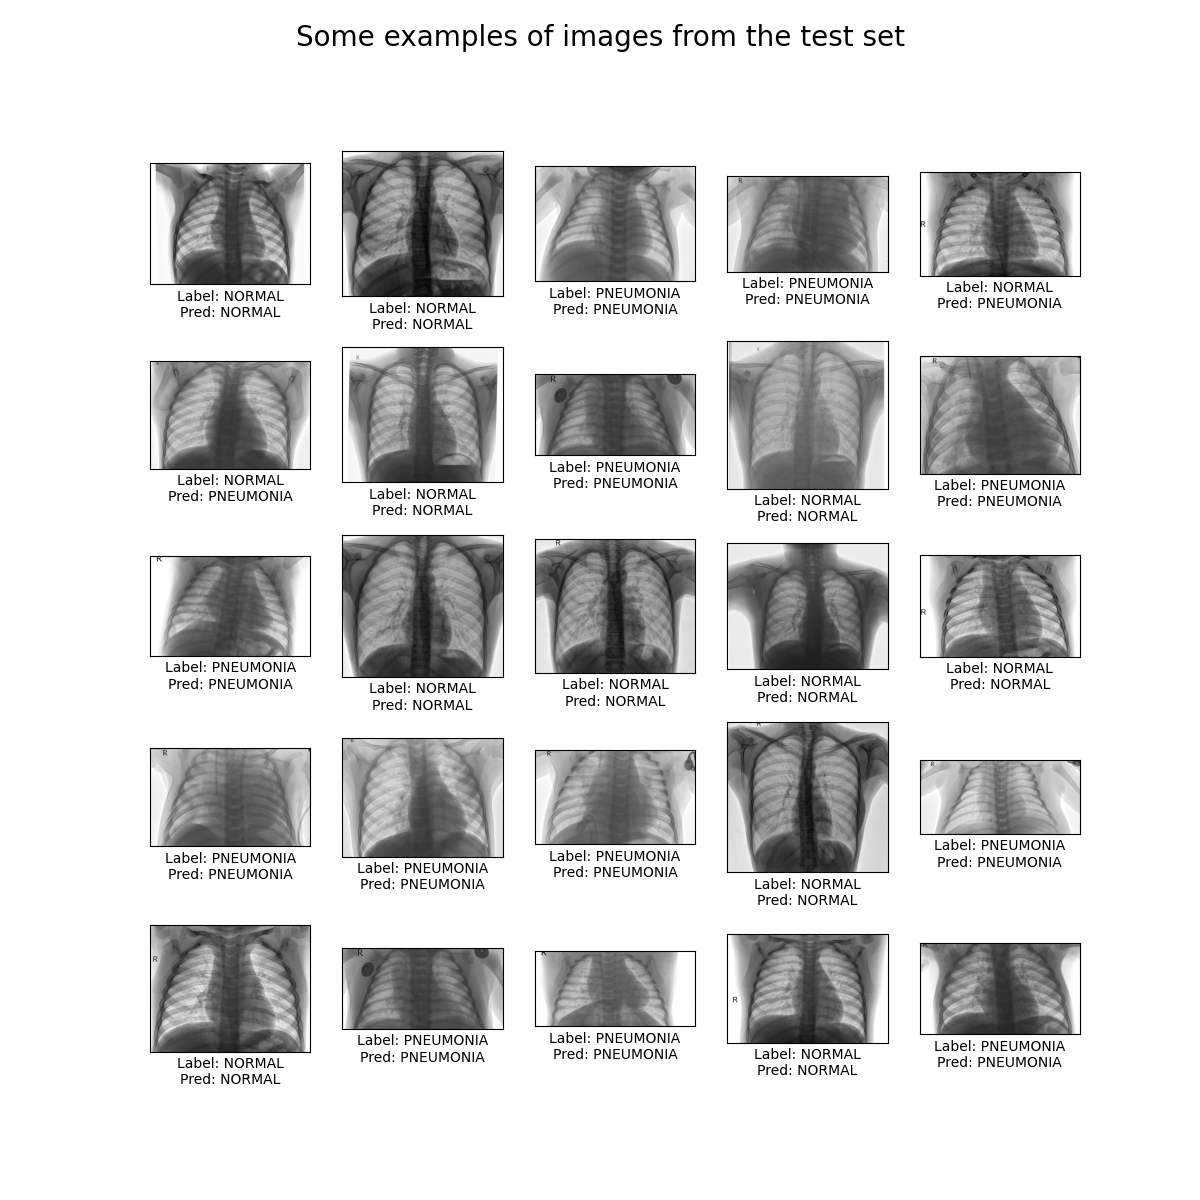
\includegraphics[width=0.5\textwidth]{./results/image/some_result.png}
  \caption{Some examples of images from the test set.}
  \label{fig:example}
\end{figure}

\section{Conclusion}
In this study, we not only established a Swim Transformer model for detecting Pneumonia in Chest X-Ray images but also enhanced its accuracy to up to 93.7\% through fine-tuning a pretrained model available on Hugging Face. This not only assists future physicians in identifying pneumonia in X-ray images but also enables the precise localization of bacterial and viral pneumonia using the object detection method of Swim Transformer in the future.

\bibliographystyle{unsrt}
\bibliography{references}

\clearpage
\section{Supplementary Material}
\subsection{Data availability}
All the data used in this analysis are publicly available, as indicated in the data tables and figures in the main text and the supplementary material. All the data used in this analysis is openly available at the following link in the GitHub repository: \url{https://github.com/CodeamonCat/2024_spring_deep_learning_for_medical_imaging_final}.

\subsection{Appendix}

\begin{figure}[!htb]
  \begin{minipage}[t]{0.45\textwidth}
    \centering
    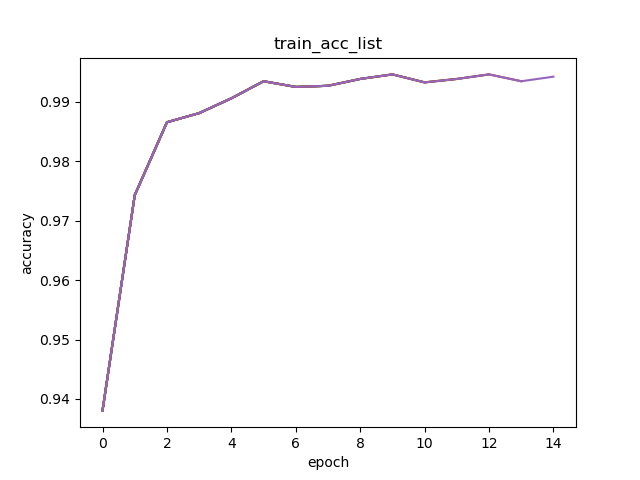
\includegraphics[width=\linewidth]{./results_train/train_acc_list.png}
    \caption{Accuracy curve of self-trained model during training.}
    \label{fig:Appendix1}
  \end{minipage}
  \hfill
  \begin{minipage}[t]{0.45\textwidth}
    \centering
    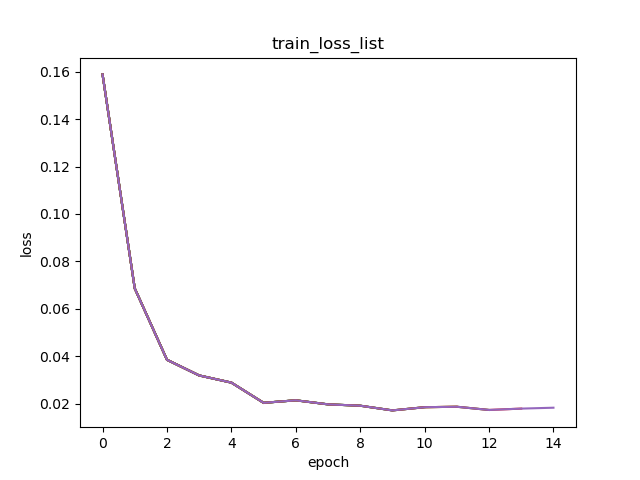
\includegraphics[width=\linewidth]{./results_train/train_loss_list.png}
    \caption{Loss curve of self-trained model during training.}
    \label{fig:Appendix2}
  \end{minipage}
\end{figure}

\begin{figure}[!htb]
  \begin{minipage}[t]{0.45\textwidth}
    \centering
    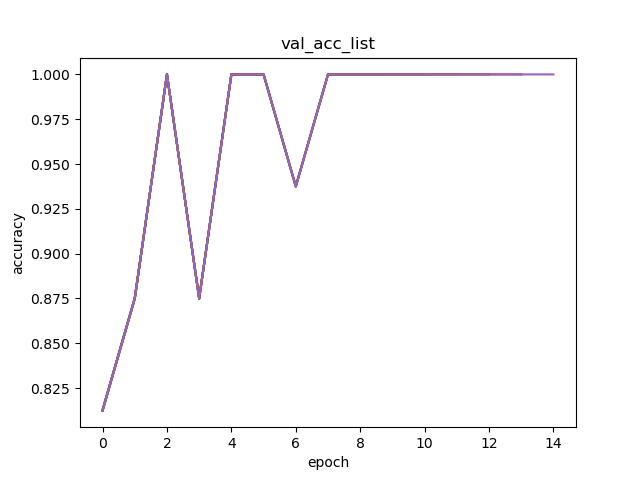
\includegraphics[width=\linewidth]{./results_train/val_acc_list.png}
    \caption{Accuracy curve of self-trained model during validation.}
    \label{fig:Appendix3}
  \end{minipage}
  \hfill
  \begin{minipage}[t]{0.45\textwidth}
    \centering
    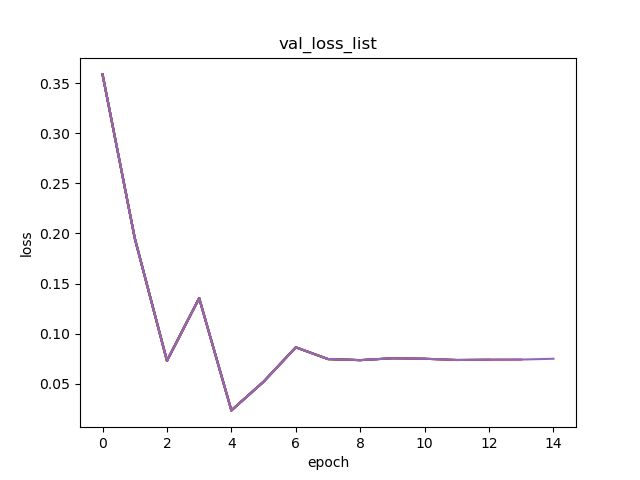
\includegraphics[width=\linewidth]{./results_train/val_loss_list.png}
    \caption{Loss curve of self-trained model during validation.}
    \label{fig:Appendix4}
  \end{minipage}
\end{figure}

\end{document}
